\chapter{Dise\~no e Implementaci\'on del prototipo}

% **************************** Define Graphics Path **************************
\ifpdf
    \graphicspath{{Chapter4/Figs/Raster/}{Chapter4/Figs/PDF/}{Chapter4/Figs/}}
\else
    \graphicspath{{Chapter4/Figs/Vector/}{Chapter4/Figs/}}
\fi

Este cap\'itulo esta destinado a la comprensi\'on de los aspectos principales que hacen al dise\~no e implementaci\'on del prototipo para la RAU2. Cabe destacar que en el mismo se toman como punto de partida las decisiones asumidas en el cap\'itulo anterior.

Por otro lado aspectos muy t\'ecnicos o problemas encontrados en cada componente de la arquitectura son tratados en profundidad en respectivos ap\'endices, citándose aquí las referencias en caso que corresponda para complementar su lectura.\\

\section[Lineamientos generales]{Lineamientos generales}

Como se menciona en el cap\'itulo destinado al estado del arte, la arquitectura del prototipo a construir esta orientada a la implementaci\'on de servicios de VPN IP/MPLS Multipunto.

Sin embargo varios aspectos de la arquitectura a\'un deben ser definidos. Es necesario definir la estrategia para calcular las rutas o caminos en la red del prototipo(algoritmo de ruteo), la forma en que se asignan y distribuyen etiquetas mpls para implementar el plano de reenvío(algoritmo de distribución de etiquetas), como se implementa la clasificaci\'on de tr\'afico y de que forma se implementan múltiples caminos para un mismo destino, ya sea para priorizar tr\'afico por tipo de aplicaci\'on por ejemplo o simplemente para hacer balanceo de carga. 

A continuaci\'on se explica de que forma el prototipo implementa cada uno de los aspectos anteriores.

\subsection{Algoritmo de Ruteo}

Una alternativa para el c\'alculo de rutas en el prototipo es utilizar protocolos de ruteo en base a IP, sacando provecho as\'i de algoritmos existentes, robustos y ampliamente probados tanto en la academia como en la industria.\\

Hist\'oricamente se han utilizado algoritmos distribuidos para el computo de rutas, siendo algunos de los m\'as renombrados en la literatura OSPF\cite{moy1998rfc}, RIP\cite{malkin1994rip} y IS-IS\cite{routingprotocol}. Por otro lado también puede sacarse provecho de la visi\'on global del plano de control de SDN para implementar un algoritmo de ruteo centralizado, sencillo y transparente.

En este trabajo se combinan ambos enfoques, utilizando el protocolo de ruteo OSPF en conjunto con un algoritmo centralizado en el controlador.\\

Se decide utilizar OSPF por la sencilla razón de que es una opción robusta y confiable, adem\'as de que existen buenas implementaciones en software libre (por ejemplo Quagga\cite{Quagga} y BIRD\cite{BIRD}).

OSPF basa su algoritmo para el c\'alculo de rutas en el algoritmo Dijkstra(ampliamente conocido para el calculo de mejores caminos en un grafo) y utiliza como m\'etrica el costo asociado a cada enlace. Este costo es ingresado manualmente por el administrador de la red y es un n\'umero \'unico, as\'i que es necesario definir una relaci\'on matem\'atica entre las diferentes caracter\'isticas de un enlace a considerar (ancho de banda disponible, tecnolog\'ia, latencia, etc.) y \'este n\'umero.

Sin embargo, para la definición de políticas en ingeniería de tr\'afico que permitan hacer balanceo de carga y construcción de caminos alternativos, es necesario incorporar m\'as informaci\'on en el algoritmo de ruteo, como la saturaci\'on de enlaces por ejemplo entre otras restricciones.

Esto es equivalente a extender OSPF para implementar un algoritmo de ruteo con restricciones, lo que en algunas implementaciones se denomina CSPF(Constrained Shortest Path First). Adem\'as interesa que estas restricciones puedan definirse dinamicamente en función de la alta y baja de servicios en el prototipo.\\

En el prototipo se ejecuta el protocolo OSPF en cada nodo y el propio controlador para construir y mantener una base de datos topol\'ogica de la red. Luego esta información es utilizada por el algoritmo de ruteo centralizado en el controlador (eventualmente CSPF) para el computo de las mejores rutas asociadas al tr\'afico de cada servicio de VPN.\\

La clasificaci\'on de tr\'afico, creación de m\'ultiples caminos y balanceo de carga son implementados en el controlador a través de una aplicaci\'on SDN, por lo que ser\'an explicados m\'as adelante en el capitulo 5.

\subsection{Algoritmo de distribución de etiquetas}

Para la implementaci\'on de un algoritmo de distribución de etiquetas, se pueden tomar también dos enfoques posibles: enfoque centralizado y enfoque distribuido.\\

Siguiendo un enfoque distribuido una de las propuestas existentes es el protocolo LDP(Label distribution Protocol), del cual adem\'as se cuenta con la implementaci\'on ofrecida por Quagga-LDP. 

Esta herramienta es una extension de Quagga, para brindar adem\'as soporte al protocolo LDP. Al igual que Quagga, el cual funciona interactuando con el kernel de Linux para la construcci\'on de la tabla de ruteo, Quagga-LDP interact\'ua con el kernel de Linux para la construcci\'on de dos tablas. Estas dos tablas implementan los conceptos de FTN (Fec To NHLFE), ILM (Incoming Label Mapping) y NHLFE (Next Hop Label Forwarding Entry) introducidos en la definición del protocolo MPLS.  Estas tablas determinan la forma en que un paquete es procesado y reenviado en un nodo.

Quagga-LDP toma como entrada el resultado de la ejecuci\'on del protocolo OSPF, para luego ejecutar el protocolo LDP y así poblar las tablas mencionadas.

Como Linux no ofrece nativamente soporte al protocolo MPLS, Quagga-LDP funciona en conjunto con MPLS-Linux; un kernel de Linux modificado para ofrecer una implementaci\'on de MPLS a nivel de kernel.\\

Utilizar Quagga-LDP y MPLS-Linux tiene dos ventajas principalmente: en primer lugar no se debe implementar un algoritmo propio con lo cual se ahorra tiempo de implementaci\'on y se tiene un algoritmo probado y confiable; en segundo lugar se disminuye la carga de computo en el controlador puesto que se ejecuta el algoritmo en cada nodo.

Por ello en este trabajo se decide probar esta alternativa y experimentar con el algoritmo de distribución de etiquetas implementado por Quagga-LDP.\\

Se dedica un tiempo considerable a la instalaci\'on de las herramientas Quagga-LDP y MPLS-Linux para lo cual es necesario recompilar diferentes versiones de kernel de Linux intentando encontrar una versi\'on apropiada para la configuración de herramientas con la que se viene trabajando en la arquitectura del prototipo. Ademas existen dos versiones bien diferentes de la implementaci\'on MPLS-Linux: una versi\'on original del año 2005 de la cual existe poca documentación y una versi\'on m\'as nueva basada en la primera que data del año 2011, de la cual se cuenta con a\'un menos documentación. 

Por un lado se prueba con ambas versiones, teniendo problemas para que el ambiente funcione correctamente (ver apéndice \ref{apendiceB6} por mayores detalles). Mientras que por otro lado se evidenci\'o dificultades para la integración entre la salida del protocolo LDP y el algoritmo de ruteo semidin\'amico definido en la sección anterior.

Por ello se decide implementar desde cero un algoritmo de distribución de etiquetas centralizado en el controlador. Los detalles de implementaci\'on del mismo ser\'an explicados m\'as adelante en la sección \ref{section5.5.4}.\\

A continuación se explica la arquitectura general del prototipo. 

\section{Construcci\'on del prototipo y Arquitectura}

La arquitectura del prototipo (ver figura ~\ref{fig:OpenSourceRArch0}), sigue la arquitectura del enfoque OpenFlow/SDN como se mencion\'o anteriormente. En concordancia con esta arquitectura en el prototipo se tienen dos componentes importantes: el controlador SDN y el switch compatible con OpenFlow.\\

En el controlador SDN se ejecuta RAUFlow, la aplicaci\'on encargada de proveer una implementaci\'on para servicios de redes privadas virtuales. A su vez esta aplicaci\'on implementa el algoritmo de ruteo  centralizado, el algoritmo de distribución de etiquetas e implementa a su vez una interfaz gr\'afica de gesti\'on para la red del prototipo.\\

\begin{figure}[htbp!] 
\centering    
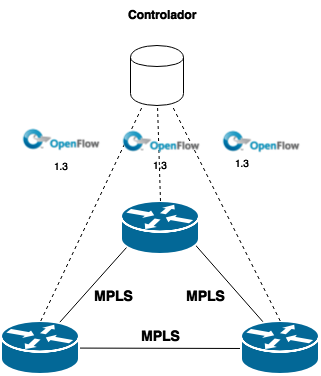
\includegraphics[width=0.4\textwidth]{Arch_Figure0}
\caption[OpenSourceRArch0]{Esquema general del prototipo}
\label{fig:OpenSourceRArch0}
\end{figure}

Por otro lado se tiene el switch compatible con el protocolo OpenFlow. Este dispositivo, denominado de aqu\'i en m\'as RAU-Switch, es implementado mediante una PC de escritorio con el hardware NetFPGA instalado y el software Open vSwitch entre otras componentes.\\ 

Para la implementaci\'on del plano de reenvío(encaminar un paquete de un nodo origen a otro destino), en cada nodo del prototipo se utilizan las tablas de flujos de OpenFlow. Mediante el esquema de flujos de OpenFlow se definen reglas de reenv\'io en base a la conmutaci\'on de etiquetas MPLS, as\'i como pol\'iticas de clasificaci\'on de tr\'afico.\\

De esta forma el prototipo para la RAU2 se compone entonces de unos pocos nodos constru\'idos en base a RAU-Switch y un controlador SDN compatible con OpenFlow, en donde se ejecuta la aplicaci\'on RAUFlow.\\

A continuaci\'on se explica en detalle cada una de estas componentes y su interacci\'on.

\section{RAU-Switch}
Cada nodo en la red del prototipo es lo que en este trabajo se denomina RAU-Switch: un switch IP/MPLS h\'ibrido compatible con OpenFlow. Por un lado es un switch OpenFlow puesto que esta dise\~nado en base a dicha arquitectura y por otro lado es un router IP/MPLS puesto que conceptualmente el plano de reenvío es implementado a trav\'es de la conmutación de etiquetas mpls, mientras que el descubrimiento de la topolog\'ia y la construccui\'on de rutas se basa en algoritmos en base a IP.\\

Puesto que en la literatura OpenFlow es común la denominación de switch OpenFlow a cualquier dispositivo, no importando si en la practica implementa las funcionalidades de un switch de capa dos \'o un router de capa tres, se decidió denominar a esta componente RAU-Switch.\\

La estructura de este dispositivo esta caracterizada por las componentes que se muestran en la figura~\ref{fig:OpenSourceRArch}.

\begin{figure}[htbp!] 
\centering    
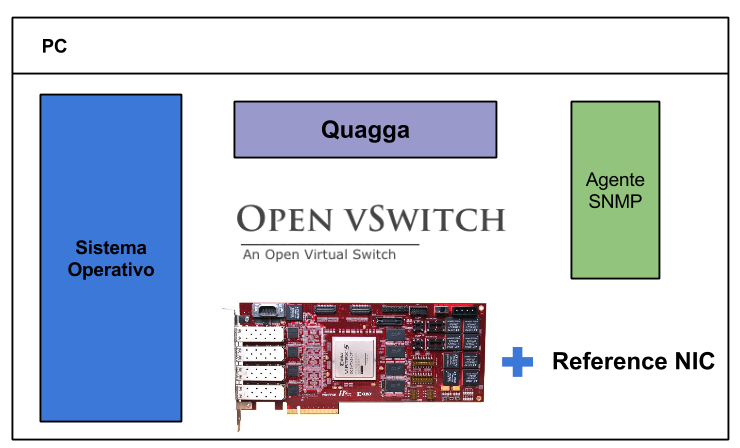
\includegraphics[width=0.7\textwidth]{Arch_Figure1}
\caption[RAU-Switch - diagrama de componentes]{RAU-Switch - diagrama de componentes}
\label{fig:OpenSourceRArch}
\end{figure}

Se utiliza una PC de escritorio como plataforma inicial a la cual se le incorpora una tarjeta NetFPGA-10G programada para que se comporte como una placa de red(proyecto ReferenceNIC) m\'as componentes adicionales de software como Open vSwitch, Quagga y un administrador SNMP. A continuaci\'on se explica en profundidad el rol de cada componente.

\subsection{Plataforma de la PC}
El switch esta constru\'ido sobre la plataforma de una PC de escritorio convencional. En particular se trabaja con un procesador Intel Core i7 de 64 bits, una Mother ASUS ROG Maximus Formula VI, 16GB de memoria DDR3, y un disco HDD de 1TB de capacidad. En el anexo \ref{annexI.1} pueden encontrarse estos detalles con mayor profundidad.

\subsection{Sistema Operativo}
En relación al sistema operativo, se decide trabajar con Ubuntu 12.04 sobre una arquitectura de 64 bits. Esta elecci\'on responde a dos criterios esencialmente: por un lado la premisa de trabajar con software libre y de c\'odigo abierto preferentemente sugiere la b\'usqueda de un sistema operativo entre alternativas basadas en GNU/Linux; por otro el hardware NetFPGA asi como los proyectos existentes para su programaci\'on fueron desarrollados trabajando sobre la plataforma Fedora14. 

Teniendo presente esto, se intenta infructuosamente instalar y configurar el hardware sobre Fedora14. Se prueba con versiones m\'as recientes de la plataforma como Fedora17 y Fedora19 obteniendo los mismos resultados; detectándose entre las causas de error, incompatibilidades entre la placa madre de la PC y las versiones de sistema operativo mencionadas y falta de drivers apropiados para cable JTag utilizado para programar el hardware. 

Finalmente tras probar con otras alternativas, se logra instalar y configurar exitosamente el hardware sobre la plataforma Ubuntu 12.04.

\subsection{Hardware NetFPGA}

El hardware NetFPGA puede funcionar tanto conectado a una PC por un slot PCIe(modo servidor), como conectado \'unicamente a una fuente de energ\'ia el\'ectrica(modo standalone). En el dise\~no planteado el hardware se encuentra conectado a la PC mediante un slot PCIe; es decir, en modo servidor.

%\subsubsection{Instaaci\'on}
%La tarjeta NetFPGA se encuentra conectada a la PC mediante un slot PCIe. Para programarla, es necesario contar con la suite de Xilinx ISE instalada correctamente, con las respectivas licencias de productos, y un cable de programaci\'on JTAG. En particular, en el prototipo cada router cuenta con la suite de Xilinx ISE instalada, habilitando su reprogramaci\'on. Notar de todos modos que no es estrictamente necesario contar con la suite de Xilinx en el router para su funcionamiento.  

\subsubsection{Herramientas de Programaci\'on}

El hardware puede programarse mediante un cable programador JTAG y la herramienta Impact de la suite de desarrollo de Xilinx ISE SDK. Para ello es indispensable contar con una estaci\'on de trabajo con dichas herramientas instaladas, habilitando la programaci\'on  de la tarjeta NetFPGA que luego ser\'a colocada en la PC de cada nodo. A su vez esta suite se compone por varias herramientas las cuales están licenciadas. Estas licencias adem\'as contemplan la arquitectura del chip Xilinx que en este caso tiene la tarjeta NetFPGA, por ello es indispensable contar con el paquete de licencias apropiado al modelo de chip con que se trabaja (en nuestro caso Virtex5) y a las herramientas utilizadas. 

Esta estaci\'on de trabajo puede o bien ser la propia PC utilizada para el switch(alternativa utilizada en este proyecto) \'o bien puede ser una PC independiente.

%Cabe destacar que en la b\'usqueda de una plataforma compatible para la programaci\'on del hardware se probo con diferentes sistemas operativos como se menciono, logrando programarse el mismo en Windows XP y Ubuntu 12.04.

\subsubsection{Programaci\'on simple}
El hardware puede programarse al menos de dos formas diferentes; una de ellas es lo que aqu\'i se denomina programaci\'on simple. Esta estrategia consiste en la utilizaci\'on de la herramienta Impact y el cable JTAG para grabar en dos chips de la tarjeta (chip FPGA y chip CPLD) dos archivos binarios, uno con la arquitectura de un proyecto y otro con la implementaci\'on del mismo.

Como principales ventajas de esta estrategia se destacan su simplicidad, no requiere de licencias pagas (puede descargarse una licencia gratuita para la herramienta Impact) y adem\'as es el procedimiento que se describe en la documentaci\'on de la plataforma NetFPGA.

No obstante presenta una desventaja importante y es que al producirse un corte de corriente el hardware se “desprograma”. Concretamente el contenido del chip FPGA se borrada y solo perdura el contenido del chip CPLD.\\

Tras constatarse este comportamiento, luego de revisar la documentaci\'on de la plataforma y recurrir al foro de la comunidad NetFPGA, se accede a una lista de correos mediante la cual se establece una comunicaci\'on con el equipo de desarrollo de NetFPGA(ver ap\'endice ~\ref{apendiceB2}). Este di\'alogo adem\'as de ayudar en la comprensión del funcionamiento de la plataforma, desemboca en la segunda estrategia de programaci\'on.

\subsubsection{Programaci\'on persistente}
El hardware NetFPGA cuenta en su arquitectura con dos unidades de memoria flash(Flash A y Flash B). En la programaci\'on persistente estas unidades se utilizan para almacenar la programaci\'on del hardware, permitiendo que en cada encendido el chip FPGA sea programado a partir del contenido de una de estas unidades. Por defecto el chip siempre se programa con el contenido de la memoria flash A, habilitando su reprogramaci\'on desde la memoria flash B v\'ia la interfaz PCIe (por mayores detalles de este procedimiento ver ~\citep{PCIEProgProject}).\\

Reprogramar el contenido del chip FPGA en tiempo de encendido, así como también mediante la interfaz PCIe requiere de módulos adicionales tanto en el contenido del chip FPGA, como en el del CPLD. En particular los proyectos ReferenceNIC\citep{ReferenceNICProject}, ReferenceSwitch~\citep{ReferenceSwitchProject} y ReferenceRouter~\citep{ReferenceRouterProject} incorporan estas características.\\

En el procedimiento empleado, inicialmente se programa el hardware con el proyecto ReferenceNIC utilizando la Programaci\'on Simple. Luego es necesario transformar la implementaci\'on del proyecto(archivo bitfile) en un archivo con el formato apropiado para ser almacenado en una de las memorias flash(archivo binario). Esto \'ultimo se realiza utilizando herramientas inclu\'idas en la plataforma de NetFPGA. Finalmente utilizando la herramienta \textbf{pcieprog} también de la plataforma se transfiere el archivo generado a una de las memorias.\\

Cabe destacar que durante la ejecuci\'on de este procedimiento se detectan algunos errores y comportamientos inesperados en el hardware. Esto es reportado al equipo de desarrollo de NetFPGA a través de la lista oficial de correos de soporte, reportándose en total dos errores. Luego de este di\'alogo se obtiene una soluci\'on a dichos errores los cuales cabe destacar que son contemplados y resueltos en la siguiente actualizaci\'on del repositorio de c\'odigo fuente. Por m\'as detalles acerca de estos errores y la forma en que son resueltos provisoriamente referirse al ap\'endice~\ref{apendiceA}.\\

Otro detalle a destacar de esta estrategia, es que la utilizaci\'on de herramientas de la suite de Xilinx requieren de licencias especiales pagas. En el marco de este proyecto se solicita apoyo en relaci\'on a este tema a docentes del Instituto de Ingeniería Eléctrica de la Facultad de Ingenieria (IIE) y a través del programa de apoyo universitario de Xilinx, en busca de una soluci\'on a este problema.

Si bien en el IIE no se trabaja con esta plataforma se obtiene de parte de este instituto asesoramiento sumamente \'util para la resoluci\'on de este obstáculo. Por otro lado a través del programa de apoyo a universidades de Xilinx se obtiene una interesante donaci\'on de licencias, posibilitando a una real explotaci\'on del hardware y de la plataforma. Por mayores detalles acerca de este problema puede consultarse el apéndice ~\ref{apendiceB3}.

\subsection{Open vSwitch}
En la arquitectura del dispositivo, Open vSwitch es el encargado de implementar el plano de datos de OpenFlow. En otras palabras es la componente que convierte mediante una implementaci\'on en software a la PC construida en un switch OpenFlow.\\

Siguiendo la especificaci\'on de OpenFlow, Open vSwitch implementa el concepto de tabla de flujos. Estas tablas(Open vSwitch implementa 256 tablas) son utilizadas por la aplicaci\'on RAUFlow para construir caminos en la topolog\'ia, instalando en forma de flujos OpenFlow las reglas de reenvío que sean necesarias en cada nodo involucrado en un camino.

Para implementar el plano de reenvío en base a la conmutaci\'on de etiquetas MPLS, se utilizan primitivas del protocolo OpenFlow, que permiten colocar y extraer etiquetas MPLS de un paquete(PUSH y POP), así como clasificar un paquete acorde al valor de la etiqueta MPLS contenida en \'el.\\

En relaci\'on a este \'ultimo punto, vale la pena destacar que la compatibilidad con estas funcionalidades del protocolo OpenFlow, están acotadas naturalmente  por la implementaci\'on de Open vSwitch. En este trabajo inicialmente se utiliza la versi\'on oficial m\'as reciente de dicha herramienta (versi\'on 2.3.1), en la cual acorde a las notas de liberaci\'on y a la secci\'on de preguntas frecuentes se garantiza soporte para solo un subconjunto de funcionalidades de la versi\'on 1.3 del protocolo OpenFlow. Entre estas funcionalidades se destacan la capacidad para match, push y pop de una \'unica etiqueta MPLS, así como su posterior procesamiento en el pipe de OpenFlow. No obstante como se explica en el apéndice ~\ref{apendiceB5} junto a otras características a destacar de Open vSwitch, este comportamiento no es el que realmente manifiesta esta versi\'on de la herramienta. En particular la operación Pop de MPLS no funciona correctamente, así como el posterior procesamiento del paquete tras manipular etiquetas acorde al pipe de OpenFlow.\\ 

Afortunadamente esta falla se encuentra reportada como error y es resuelta en la versi\'on de desarrollo~\citep{OVSSourceCode}, la cual a su vez tras instalarse se comprueba que soporta match, push y pop de hasta tres etiquetas mpls, junto el posterior procesamiento del paquete. De esta forma la versi\'on de Open vSwitch utilizada es la de desarrollo.\\

Por otro lado, resulta interesante a tener en consideraci\'on que las operaciones de match, push y pop de MPLS son implementadas en modo usuario.

%Por otro lado en relaci\'on a las componentes de software, el router se compone de un sistema operativo escritorio basado en linux, con las instalaciones de Open vSwitch, Quagga y el agente de gesti\'on SNMP. Nuevamente por mayores detalles acerca de las versiones de software utilizadas, sistema operativo entre otros detalles refierase al anexo [link al anexo].\\

\subsection{Quagga}
En cada nodo se ejecuta una instancia del software de enrutamiento Quagga, configurada para ejecutar el demonio ospf.\\ 

El demonio ospf implementa el protocolo de igual nombre y se utiliza para obtener información de cada nodo y sus adyacencias en la topolog\'ia, guardando dicha información en una base de datos local(Link-State-Database o LSDB). Entre los datos que se incluyen en esta base de datos topol\'ogica se destaca por ejemplo el costo asociado a cada adyacencia.\\ 

Como se menciona anteriormente, el algoritmo OSPF utiliza solamente para la construcci\'on de la base de datos topol\'ogica. Si bien en un inicio se piensa en trabajar con la salida de dicho algoritmo, finalmente se decidió trabajar con el algoritmo de ruteo centralizado implementado en el controlador. Por ello en la versi\'on final del prototipo no se utiliza la salida de este algoritmo a pesar de que la arquitectura permite su utilización para alimentar la entrada de procesos que se ejecuten en el controlador.\\

De esta forma cada switch del prototipo así como el propio controlador ejecuta una instancia de Quagga con el demonio ospf configurado como se muestra en el apéndice \ref{appendix4}. Cabe destacar de dicha configuración que la adyacencia entre un switch y el Controlador(enlace utilizado para el canal de comunicación OpenFlow) tiene asociado costo infinito para evitar que sea utilizado tanto por el algoritmo OSPF como por el algoritmo CSPF en la construcción de algún camino. En la implementaci\'on de Quagga el costo infinito es representado por el numero 65535(16 bits).

\subsection{Agente SNMP}
El protocolo de comunicación OpenFlow dentro de las estructuras de datos utilizadas para el intercambio de información entre un switch y el Controlador, no prevee una forma de comunicar el direccionamiento IP propio del equipo (direcciones IP de cada interfaz física). En particular la estructura \textit{ofp\_port} utilizada por el mensaje \textit{OFPMP\_PORT\_DESCRIPTION} no provee de dicho campo (ver especificación del protocolo OpenFlow 1.3\citep{ofv133spec}). Por esta razón es necesaria una forma de comunicar al controlador información adicional sobre características de cada nodo como la dirección IP de una interfaz, que no puede ser enviada a través del protocolo OpenFlow. Para evitar modificar el protocolo extendiéndolo para comunicar dicha informaci\'on, se utiliza un agente SNMP.\\

SNMP definido a través de los RFC1065~\citep{rose1990structure} y RFC1157~\citep{case1989simple} entre otros, es un protocolo que permite intercambio de información entre dispositivos de red y una entidad administradora. Para su despliegue en una red son necesarias tres componentes: 

\begin{enumerate}

\item Dispositivo administrado: Es el dispositivo de red que se quiere monitorear.

\item Agente: Es el software que se ejecuta en el dispositivo administrado y se encarga de comunicarse mediante el protocolo con el sistema administrador de red.

\item Sistema administrador de red: El dispositivo que se encargara de realizar las consultas sobre la información deseada a los dispositivos administrados.

\end{enumerate}	

En el prototipo se instala un agente SNMP en cada switch (dispositivo administrado), para enviar la correspondencia entre números de puerto OpenFlow y direcciones IP al Controlador(sistema administrador).\\

No es el objetivo de este trabajo entrar en detalle sobre el protocolo SNMP por lo que si el lector desea profundizar en estos conceptos se recomienda seguir las referencia mencionadas anteriormente.

\section{Entidad Controlador}
Como se muestra en \ref{fig:OpenSourceRArch0} cada nodo del prototipo responde a una entidad denominada Controlador. Esta entidad en la pr\'actica es una PC convencional con determinadas componentes de software(ver figura \ref{fig:OpenSourceRArch3}) entre las cuales se destaca el controlador SDN Ryu, pilar fundamental en la implemenatci\'on de la aplicaci\'on RAUFlow. A su vez se encuentran los módulos Administrador SNMP utilizado en la comunicaci\'on con los agentes SNMP instalados en cada nodo RAUSwitch del dispositivo y LSDBSync utilizado en el proceso de extracci\'on de informaci\'on de la base de datos topol\'ogica de Quagga. 

Estas tres componentes se ejecutan en una PC de escritorio con Ubuntu 12.04 como sistema operativo. \\

A continuación se explica en detalle cada una de las tres componentes mencionadas.

\newpage
\begin{figure}[htbp!] 
\centering    
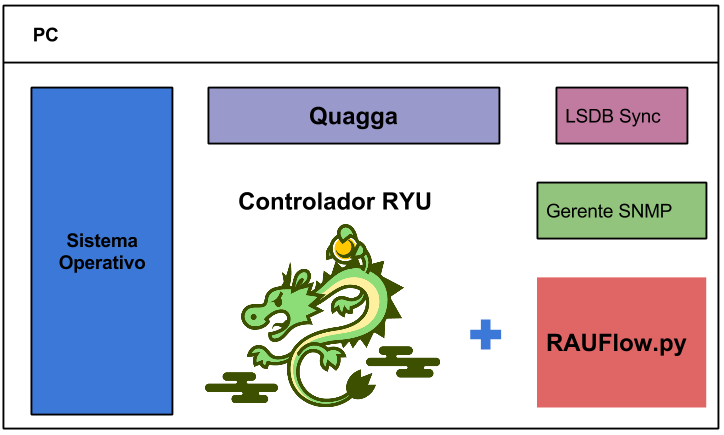
\includegraphics[width=0.6\textwidth]{Arch_Figure3}
\caption[OpenSourceRArch3]{Diagrama de componentes del Controlador}
\label{fig:OpenSourceRArch3}
\end{figure}


\subsection{Controlador Ryu}
Ryu es la alternativa de software elegido para implementar el controlador SDN compatible con el protocolo OpenFlow. 

Utilizando este herramienta para la construcci\'on y ejecuci\'on de una o m\'as aplicaciones SDN, se implementa el prácticamente la totalidad del plano de control del prototipo. Esto es en otras palabras la implementaci\'on del modelado de la realidad, la implementaci\'on de funcionalidades para la creaci\'on de servicios de redes privadas, implementaci\'on de cliasficiaci\'on de tr\'afico y eventualmente la implementaci\'on de pol\'iticas de ingenieria de tr\'afico y calidad de servicios (QoS).\\ 

Dada la complejidad en el diseño y arquitectura de esta componente, se destina íntegramente el próximo cap\'itulo a la explicaci\'on de las diferentes características e implementaci\'on de esta la o las aplicaciones Ryu que constituyen el plano de control del prototipo, as\'i como la interacci\'on de las otras componentes mencionadas dentro del plano de control como los m\'odulos LSDBSync y Administrador SNMP. 

\subsection{Quagga}
Como se menciona anteriormente, el controlador ejecuta una instancia de Quagga, obteniendo de esta forma acceso local a la información de la base de datos topol\'ogica construida por OSPF (Link-State-Database), una vez que el algoritmo converge.

Para obtener esta informaci\'on, as\'i como tambi\'en detectar cuando cambia la topolog\'ia se utiliza el siguiente m\'odulo, LSDB Sync.

\subsection{LSDB Sync}
LSDB Sync se encarga de tomar la información de la base de datos topol\'ogica una vez que el algoritmo OSPF converge, procesarla y enviarla a las aplicaciones que se ejecutan en el controlador.\\

Esta componente consta de dos módulos. El primero se encarga de escuchar los mensajes del protocolo que enviados por Quagga, generando un evento cuando el mismo reconverge, luego de producirse un cambio en la topolog\'ia; el cual luego es tomado por el segundo m\'odulo.

Una vez capturado el evento anterior, el segundo m\'odulo toma la información topol\'ogica en la base local del controlador y la procesa para ser enviada a las aplicaciones en el controlador.

Luego se produce un proceso de actualizaci\'on topol\'ogica, en el que eventualmente el controlador utilizando el m\'odulo Administrador SNMP obtiene informaci\'on adicional sobre los dispositivos del prototipo. 

\begin{subsection}{Administrador SNMP}
El administrador SNMP es utilizado para consultar al agente SNMP instalado en un nodo particular, por la correspondencia entre números de puerto OpenFlow y direcciones IP. Esta componente es utilizada por las aplicaciones en el Controlador cada vez que es preciso obtener esta información de mapeo para un nodo en particular(por ejemplo en el proceso de actualización de la topolog\'ia).\\\\\

\end{subsection}

En resumen, el prototipo se compone de nodos construidos en base al hardware NetFPGA y una PC convencional el la cual se instalan diferentes componentes de software de forma de implementar un switch MPLS/OpenFlow. Luego una PC normal en la que se instala el controlador Ryu m\'as un conjunto de m\'odulos adicionales. Como se muestra en la figura\ref{fig:OpenSourceRArch4}, luego la comunicación entre cada par de nodos es IP/MPLS, mientras que cada nodo es manipulado por el protocolo OpenFlow. Adicionalmente se tiene un canal IP entre cada nodo y el plano de control por donde se comunican cada agente SNMP con el administrador.

\newpage
\begin{figure}[Ht!] 
\centering    
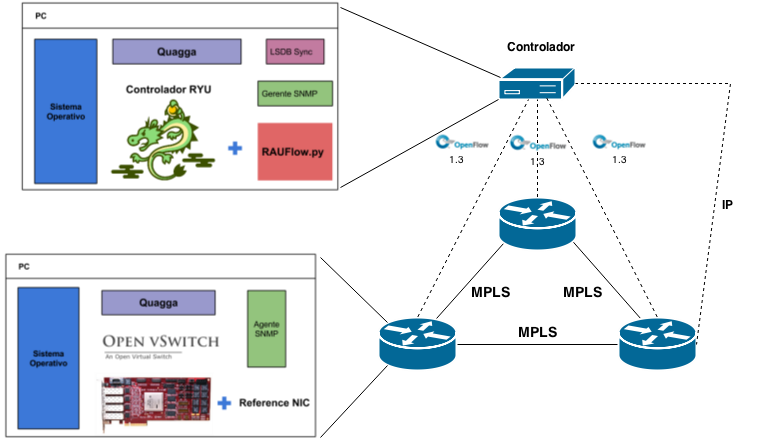
\includegraphics[width=0.9\textwidth]{Arch_Figure4}
\caption[Vista l\'ogica ampliada del prototipo]{Vista l\'ogica ampliada del prototipo}
\label{fig:OpenSourceRArch4}
\end{figure}

En el siguiente cap\'itulo se explica en detalle el proceso de diseño e implementaci\'on de la aplicaci\'on RAUFlow, as\'i como la interaci\'on con las diferentes componentes de RAUSwitch.
